The current-voltage characteristic is fundamental to understanding PV
device performance. It is a graphical representation of the relationship
between the current \(I\) and voltage \(V\) of a PV device and is often
abbreviated as the I-V characteristic or I-V curve.
Figure \ref{fig:Surfclub_IV_and_PV_curve_at_STC} shows the I-V characteristic of
a 330-watt photovoltaic module alongside its corresponding power-voltage
(P-V) curve under Standard Test Conditions. Standard Test Conditions (STC),
sometimes also referred to as Standard Rating Conditions (SRC), denote
an industry-standard set of operating conditions under which manufacturers
test the performance of their photovoltaic modules and report the results
in datasheets. These conditions specify a cell temperature of \(T = 298.15 \, \si{\kelvin}\)
and an incident irradiance of \(G_{\text{ref}} = 1000 \, \si{\watt\per\meter\squared}\) with an
air mass 1.5 solar spectrum. The figure also highlights three
important points of the I-V graph:

\begin{itemize}
    \item the open circuit point \((V = V_{oc}, I = 0,)\): The intersection with the voltage axis when
        the current is zero, representing the maximum voltage the module can produce under open-circuit conditions.
    \item the short circuit point \((V = 0, I = I_{sc})\): The intersection with the current axis when
        the voltage is zero, representing the maximum current the module can produce under short-circuit conditions.
    \item the maximum power point \((V = V_{mp}, I = I_{mp})\): The point for which the product of
        the current \(I\) and voltage \(V\) is maximized. The maximum power is given by \(P_{mp} = V_{mp} I_{mp}\).
\end{itemize}

Most modern PV module datasheets provide information on
these three points under Standard Test Conditions (STC),
and in some cases, even include the entire I-V curve. As
will be seen in Section \ref{sec:Five_parameter_model},
which presents the five-parameter model used in this thesis,
this information, along with other data from the module
datasheet, is used to calculate the model parameters.

As might be expected, only a single point from
the simulated I-V characteristic is needed to formulate a
prediction for a PV device. Ideally, this point corresponds
to the true operating point of the device, that is, the point
on the I-V curve at which the PV device operates at a
given instant. The last section of this chapter will
demonstrate how this point is chosen under certain
assumptions appropriate for PV system modeling.

All mathematical models presented in Section
\ref{sec:Background to physical models}, except for the
ideal model, are implicit, meaning they cannot be solved
explicitly for either \(I\) or \(V\). In these cases, the I-V
characteristic can be interpreted as the zero-level
set \(f_{\kappa}(V, I) = 0\)  of an appropriately defined
function \(f_{\kappa}: \mathbb{R}^2 \rightarrow \mathbb{R}\),
constrained to the upper right quadrant of the I-V plane.
The set \(\kappa\) represents the model parameters, some of
which are constant, while others depend on the operating
conditions as mentioned in Section \ref{sec:Background to physical models}.

\begin{figure}[H]
    \centering
    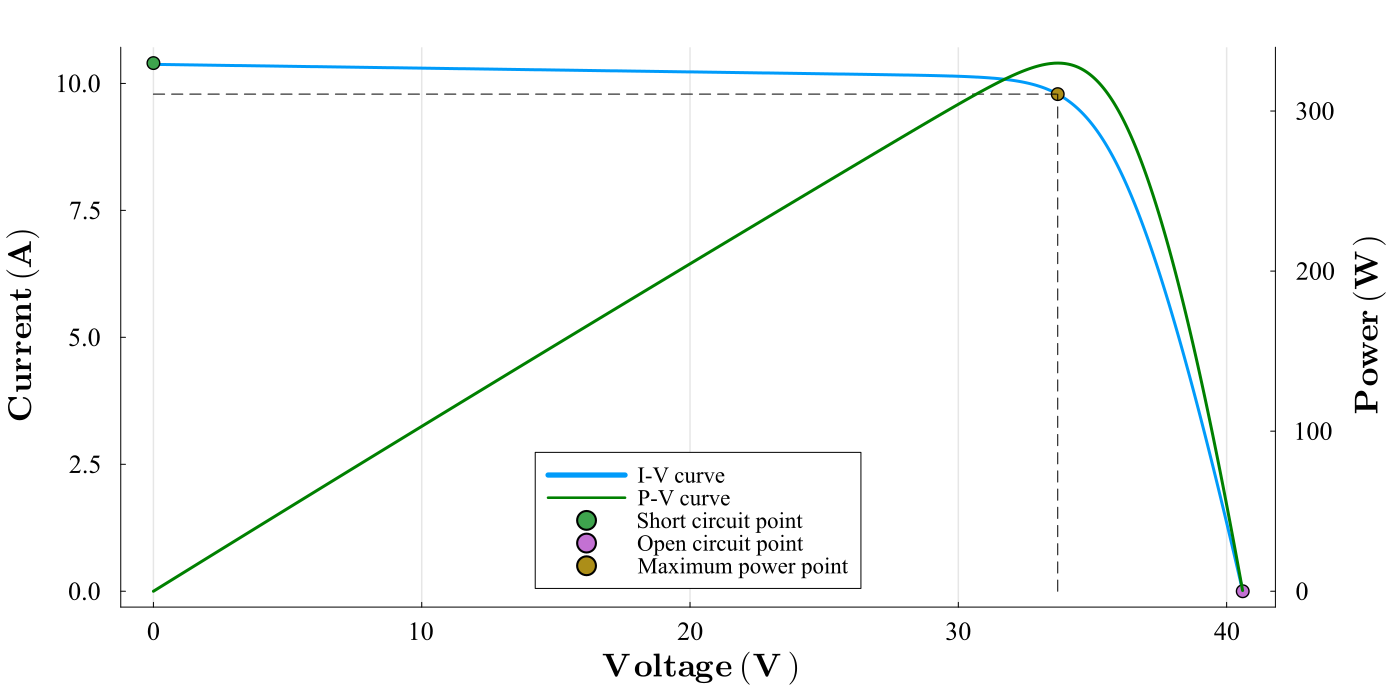
\includegraphics[scale=0.3]{Surfclub_IV_and_PV_curve_at_STC.png}
    \caption{\small Current-voltage characteristic and corresponding power-voltage curves of a photovoltaic module at STC.}
    \label{fig:Surfclub_IV_and_PV_curve_at_STC}
\end{figure}
